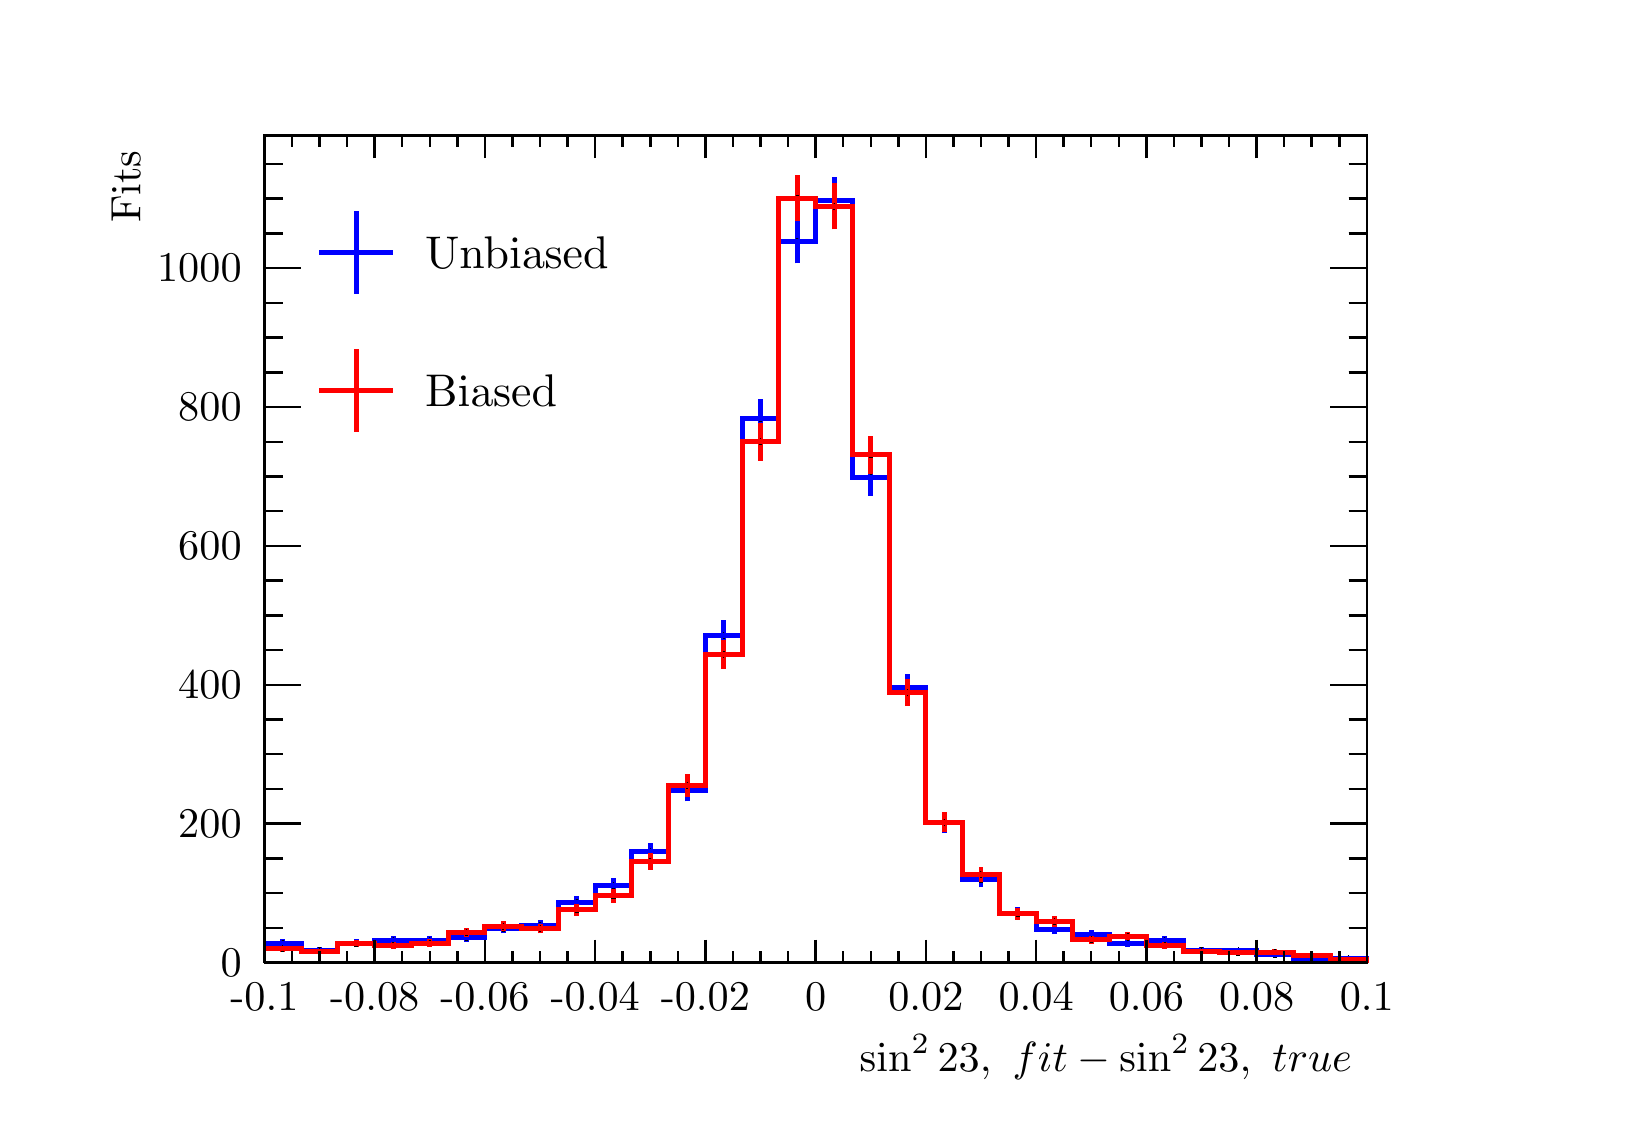
\begin{tikzpicture}
\pgfdeclareplotmark{cross} {
\pgfpathmoveto{\pgfpoint{-0.3\pgfplotmarksize}{\pgfplotmarksize}}
\pgfpathlineto{\pgfpoint{+0.3\pgfplotmarksize}{\pgfplotmarksize}}
\pgfpathlineto{\pgfpoint{+0.3\pgfplotmarksize}{0.3\pgfplotmarksize}}
\pgfpathlineto{\pgfpoint{+1\pgfplotmarksize}{0.3\pgfplotmarksize}}
\pgfpathlineto{\pgfpoint{+1\pgfplotmarksize}{-0.3\pgfplotmarksize}}
\pgfpathlineto{\pgfpoint{+0.3\pgfplotmarksize}{-0.3\pgfplotmarksize}}
\pgfpathlineto{\pgfpoint{+0.3\pgfplotmarksize}{-1.\pgfplotmarksize}}
\pgfpathlineto{\pgfpoint{-0.3\pgfplotmarksize}{-1.\pgfplotmarksize}}
\pgfpathlineto{\pgfpoint{-0.3\pgfplotmarksize}{-0.3\pgfplotmarksize}}
\pgfpathlineto{\pgfpoint{-1.\pgfplotmarksize}{-0.3\pgfplotmarksize}}
\pgfpathlineto{\pgfpoint{-1.\pgfplotmarksize}{0.3\pgfplotmarksize}}
\pgfpathlineto{\pgfpoint{-0.3\pgfplotmarksize}{0.3\pgfplotmarksize}}
\pgfpathclose
\pgfusepathqstroke
}
\pgfdeclareplotmark{cross*} {
\pgfpathmoveto{\pgfpoint{-0.3\pgfplotmarksize}{\pgfplotmarksize}}
\pgfpathlineto{\pgfpoint{+0.3\pgfplotmarksize}{\pgfplotmarksize}}
\pgfpathlineto{\pgfpoint{+0.3\pgfplotmarksize}{0.3\pgfplotmarksize}}
\pgfpathlineto{\pgfpoint{+1\pgfplotmarksize}{0.3\pgfplotmarksize}}
\pgfpathlineto{\pgfpoint{+1\pgfplotmarksize}{-0.3\pgfplotmarksize}}
\pgfpathlineto{\pgfpoint{+0.3\pgfplotmarksize}{-0.3\pgfplotmarksize}}
\pgfpathlineto{\pgfpoint{+0.3\pgfplotmarksize}{-1.\pgfplotmarksize}}
\pgfpathlineto{\pgfpoint{-0.3\pgfplotmarksize}{-1.\pgfplotmarksize}}
\pgfpathlineto{\pgfpoint{-0.3\pgfplotmarksize}{-0.3\pgfplotmarksize}}
\pgfpathlineto{\pgfpoint{-1.\pgfplotmarksize}{-0.3\pgfplotmarksize}}
\pgfpathlineto{\pgfpoint{-1.\pgfplotmarksize}{0.3\pgfplotmarksize}}
\pgfpathlineto{\pgfpoint{-0.3\pgfplotmarksize}{0.3\pgfplotmarksize}}
\pgfpathclose
\pgfusepathqfillstroke
}
\pgfdeclareplotmark{newstar} {
\pgfpathmoveto{\pgfqpoint{0pt}{\pgfplotmarksize}}
\pgfpathlineto{\pgfqpointpolar{44}{0.5\pgfplotmarksize}}
\pgfpathlineto{\pgfqpointpolar{18}{\pgfplotmarksize}}
\pgfpathlineto{\pgfqpointpolar{-20}{0.5\pgfplotmarksize}}
\pgfpathlineto{\pgfqpointpolar{-54}{\pgfplotmarksize}}
\pgfpathlineto{\pgfqpointpolar{-90}{0.5\pgfplotmarksize}}
\pgfpathlineto{\pgfqpointpolar{234}{\pgfplotmarksize}}
\pgfpathlineto{\pgfqpointpolar{198}{0.5\pgfplotmarksize}}
\pgfpathlineto{\pgfqpointpolar{162}{\pgfplotmarksize}}
\pgfpathlineto{\pgfqpointpolar{134}{0.5\pgfplotmarksize}}
\pgfpathclose
\pgfusepathqstroke
}
\pgfdeclareplotmark{newstar*} {
\pgfpathmoveto{\pgfqpoint{0pt}{\pgfplotmarksize}}
\pgfpathlineto{\pgfqpointpolar{44}{0.5\pgfplotmarksize}}
\pgfpathlineto{\pgfqpointpolar{18}{\pgfplotmarksize}}
\pgfpathlineto{\pgfqpointpolar{-20}{0.5\pgfplotmarksize}}
\pgfpathlineto{\pgfqpointpolar{-54}{\pgfplotmarksize}}
\pgfpathlineto{\pgfqpointpolar{-90}{0.5\pgfplotmarksize}}
\pgfpathlineto{\pgfqpointpolar{234}{\pgfplotmarksize}}
\pgfpathlineto{\pgfqpointpolar{198}{0.5\pgfplotmarksize}}
\pgfpathlineto{\pgfqpointpolar{162}{\pgfplotmarksize}}
\pgfpathlineto{\pgfqpointpolar{134}{0.5\pgfplotmarksize}}
\pgfpathclose
\pgfusepathqfillstroke
}
\definecolor{c}{rgb}{1,1,1};
\draw [color=c, fill=c] (0,0) rectangle (20,13.639);
\draw [color=c, fill=c] (3,1.77307) rectangle (17,12.2751);
\definecolor{c}{rgb}{0,0,0};
\draw [c,line width=0.9] (3,1.77307) -- (3,12.2751) -- (17,12.2751) -- (17,1.77307) -- (3,1.77307);
\definecolor{c}{rgb}{1,1,1};
\draw [color=c, fill=c] (3,1.77307) rectangle (17,12.2751);
\definecolor{c}{rgb}{0,0,0};
\draw [c,line width=0.9] (3,1.77307) -- (3,12.2751) -- (17,12.2751) -- (17,1.77307) -- (3,1.77307);
\draw [c,line width=0.9] (3,1.77307) -- (3.46667,1.77307) -- (3.46667,1.77307) -- (3.93333,1.77307) -- (3.93333,1.77307) -- (4.4,1.77307) -- (4.4,1.77307) -- (4.86667,1.77307) -- (4.86667,1.77307) -- (5.33333,1.77307) -- (5.33333,1.77307) --
 (5.8,1.77307) -- (5.8,1.77307) -- (6.26667,1.77307) -- (6.26667,1.77307) -- (6.73333,1.77307) -- (6.73333,1.77307) -- (7.2,1.77307) -- (7.2,1.77307) -- (7.66667,1.77307) -- (7.66667,1.77307) -- (8.13333,1.77307) -- (8.13333,1.77307) -- (8.6,1.77307)
 -- (8.6,1.77307) -- (9.06667,1.77307) -- (9.06667,1.77307) -- (9.53333,1.77307) -- (9.53333,1.77307) -- (10,1.77307) -- (10,1.77307) -- (10.4667,1.77307) -- (10.4667,1.77307) -- (10.9333,1.77307) -- (10.9333,1.77307) -- (11.4,1.77307) --
 (11.4,1.77307) -- (11.8667,1.77307) -- (11.8667,1.77307) -- (12.3333,1.77307) -- (12.3333,1.77307) -- (12.8,1.77307) -- (12.8,1.77307) -- (13.2667,1.77307) -- (13.2667,1.77307) -- (13.7333,1.77307) -- (13.7333,1.77307) -- (14.2,1.77307) --
 (14.2,1.77307) -- (14.6667,1.77307) -- (14.6667,1.77307) -- (15.1333,1.77307) -- (15.1333,1.77307) -- (15.6,1.77307) -- (15.6,1.77307) -- (16.0667,1.77307) -- (16.0667,1.77307) -- (16.5333,1.77307) -- (16.5333,1.77307) -- (17,1.77307) --
 (17,1.77307);
\draw [c,line width=0.9] (3,1.77307) -- (17,1.77307);
\draw [c,line width=0.9] (3,2.05948) -- (3,1.77307);
\draw [c,line width=0.9] (3.35,1.91628) -- (3.35,1.77307);
\draw [c,line width=0.9] (3.7,1.91628) -- (3.7,1.77307);
\draw [c,line width=0.9] (4.05,1.91628) -- (4.05,1.77307);
\draw [c,line width=0.9] (4.4,2.05948) -- (4.4,1.77307);
\draw [c,line width=0.9] (4.75,1.91628) -- (4.75,1.77307);
\draw [c,line width=0.9] (5.1,1.91628) -- (5.1,1.77307);
\draw [c,line width=0.9] (5.45,1.91628) -- (5.45,1.77307);
\draw [c,line width=0.9] (5.8,2.05948) -- (5.8,1.77307);
\draw [c,line width=0.9] (6.15,1.91628) -- (6.15,1.77307);
\draw [c,line width=0.9] (6.5,1.91628) -- (6.5,1.77307);
\draw [c,line width=0.9] (6.85,1.91628) -- (6.85,1.77307);
\draw [c,line width=0.9] (7.2,2.05948) -- (7.2,1.77307);
\draw [c,line width=0.9] (7.55,1.91628) -- (7.55,1.77307);
\draw [c,line width=0.9] (7.9,1.91628) -- (7.9,1.77307);
\draw [c,line width=0.9] (8.25,1.91628) -- (8.25,1.77307);
\draw [c,line width=0.9] (8.6,2.05948) -- (8.6,1.77307);
\draw [c,line width=0.9] (8.95,1.91628) -- (8.95,1.77307);
\draw [c,line width=0.9] (9.3,1.91628) -- (9.3,1.77307);
\draw [c,line width=0.9] (9.65,1.91628) -- (9.65,1.77307);
\draw [c,line width=0.9] (10,2.05948) -- (10,1.77307);
\draw [c,line width=0.9] (10.35,1.91628) -- (10.35,1.77307);
\draw [c,line width=0.9] (10.7,1.91628) -- (10.7,1.77307);
\draw [c,line width=0.9] (11.05,1.91628) -- (11.05,1.77307);
\draw [c,line width=0.9] (11.4,2.05948) -- (11.4,1.77307);
\draw [c,line width=0.9] (11.75,1.91628) -- (11.75,1.77307);
\draw [c,line width=0.9] (12.1,1.91628) -- (12.1,1.77307);
\draw [c,line width=0.9] (12.45,1.91628) -- (12.45,1.77307);
\draw [c,line width=0.9] (12.8,2.05948) -- (12.8,1.77307);
\draw [c,line width=0.9] (13.15,1.91628) -- (13.15,1.77307);
\draw [c,line width=0.9] (13.5,1.91628) -- (13.5,1.77307);
\draw [c,line width=0.9] (13.85,1.91628) -- (13.85,1.77307);
\draw [c,line width=0.9] (14.2,2.05948) -- (14.2,1.77307);
\draw [c,line width=0.9] (14.55,1.91628) -- (14.55,1.77307);
\draw [c,line width=0.9] (14.9,1.91628) -- (14.9,1.77307);
\draw [c,line width=0.9] (15.25,1.91628) -- (15.25,1.77307);
\draw [c,line width=0.9] (15.6,2.05948) -- (15.6,1.77307);
\draw [c,line width=0.9] (15.95,1.91628) -- (15.95,1.77307);
\draw [c,line width=0.9] (16.3,1.91628) -- (16.3,1.77307);
\draw [c,line width=0.9] (16.65,1.91628) -- (16.65,1.77307);
\draw [c,line width=0.9] (17,2.05948) -- (17,1.77307);
\draw [c,line width=0.9] (3,2.05948) -- (3,1.77307);
\draw [c,line width=0.9] (17,2.05948) -- (17,1.77307);
\draw [anchor=base] (3,1.15931) node[scale=1.52731, color=c, rotate=0]{-0.1};
\draw [anchor=base] (4.4,1.15931) node[scale=1.52731, color=c, rotate=0]{-0.08};
\draw [anchor=base] (5.8,1.15931) node[scale=1.52731, color=c, rotate=0]{-0.06};
\draw [anchor=base] (7.2,1.15931) node[scale=1.52731, color=c, rotate=0]{-0.04};
\draw [anchor=base] (8.6,1.15931) node[scale=1.52731, color=c, rotate=0]{-0.02};
\draw [anchor=base] (10,1.15931) node[scale=1.52731, color=c, rotate=0]{0};
\draw [anchor=base] (11.4,1.15931) node[scale=1.52731, color=c, rotate=0]{0.02};
\draw [anchor=base] (12.8,1.15931) node[scale=1.52731, color=c, rotate=0]{0.04};
\draw [anchor=base] (14.2,1.15931) node[scale=1.52731, color=c, rotate=0]{0.06};
\draw [anchor=base] (15.6,1.15931) node[scale=1.52731, color=c, rotate=0]{0.08};
\draw [anchor=base] (17,1.15931) node[scale=1.52731, color=c, rotate=0]{0.1};
\draw [anchor= east] (17,0.572837) node[scale=1.52731, color=c, rotate=0]{$\sin^{2}\thetai{23,~\text{fit}} - \sin^{2}\thetai{23,~\text{true}}$};
\draw [c,line width=0.9] (3,12.2751) -- (17,12.2751);
\draw [c,line width=0.9] (3,11.9887) -- (3,12.2751);
\draw [c,line width=0.9] (3.35,12.1319) -- (3.35,12.2751);
\draw [c,line width=0.9] (3.7,12.1319) -- (3.7,12.2751);
\draw [c,line width=0.9] (4.05,12.1319) -- (4.05,12.2751);
\draw [c,line width=0.9] (4.4,11.9887) -- (4.4,12.2751);
\draw [c,line width=0.9] (4.75,12.1319) -- (4.75,12.2751);
\draw [c,line width=0.9] (5.1,12.1319) -- (5.1,12.2751);
\draw [c,line width=0.9] (5.45,12.1319) -- (5.45,12.2751);
\draw [c,line width=0.9] (5.8,11.9887) -- (5.8,12.2751);
\draw [c,line width=0.9] (6.15,12.1319) -- (6.15,12.2751);
\draw [c,line width=0.9] (6.5,12.1319) -- (6.5,12.2751);
\draw [c,line width=0.9] (6.85,12.1319) -- (6.85,12.2751);
\draw [c,line width=0.9] (7.2,11.9887) -- (7.2,12.2751);
\draw [c,line width=0.9] (7.55,12.1319) -- (7.55,12.2751);
\draw [c,line width=0.9] (7.9,12.1319) -- (7.9,12.2751);
\draw [c,line width=0.9] (8.25,12.1319) -- (8.25,12.2751);
\draw [c,line width=0.9] (8.6,11.9887) -- (8.6,12.2751);
\draw [c,line width=0.9] (8.95,12.1319) -- (8.95,12.2751);
\draw [c,line width=0.9] (9.3,12.1319) -- (9.3,12.2751);
\draw [c,line width=0.9] (9.65,12.1319) -- (9.65,12.2751);
\draw [c,line width=0.9] (10,11.9887) -- (10,12.2751);
\draw [c,line width=0.9] (10.35,12.1319) -- (10.35,12.2751);
\draw [c,line width=0.9] (10.7,12.1319) -- (10.7,12.2751);
\draw [c,line width=0.9] (11.05,12.1319) -- (11.05,12.2751);
\draw [c,line width=0.9] (11.4,11.9887) -- (11.4,12.2751);
\draw [c,line width=0.9] (11.75,12.1319) -- (11.75,12.2751);
\draw [c,line width=0.9] (12.1,12.1319) -- (12.1,12.2751);
\draw [c,line width=0.9] (12.45,12.1319) -- (12.45,12.2751);
\draw [c,line width=0.9] (12.8,11.9887) -- (12.8,12.2751);
\draw [c,line width=0.9] (13.15,12.1319) -- (13.15,12.2751);
\draw [c,line width=0.9] (13.5,12.1319) -- (13.5,12.2751);
\draw [c,line width=0.9] (13.85,12.1319) -- (13.85,12.2751);
\draw [c,line width=0.9] (14.2,11.9887) -- (14.2,12.2751);
\draw [c,line width=0.9] (14.55,12.1319) -- (14.55,12.2751);
\draw [c,line width=0.9] (14.9,12.1319) -- (14.9,12.2751);
\draw [c,line width=0.9] (15.25,12.1319) -- (15.25,12.2751);
\draw [c,line width=0.9] (15.6,11.9887) -- (15.6,12.2751);
\draw [c,line width=0.9] (15.95,12.1319) -- (15.95,12.2751);
\draw [c,line width=0.9] (16.3,12.1319) -- (16.3,12.2751);
\draw [c,line width=0.9] (16.65,12.1319) -- (16.65,12.2751);
\draw [c,line width=0.9] (17,11.9887) -- (17,12.2751);
\draw [c,line width=0.9] (3,11.9887) -- (3,12.2751);
\draw [c,line width=0.9] (17,11.9887) -- (17,12.2751);
\draw [c,line width=0.9] (3,1.77307) -- (3,12.2751);
\draw [c,line width=0.9] (3.462,1.77307) -- (3,1.77307);
\draw [c,line width=0.9] (3.231,2.214) -- (3,2.214);
\draw [c,line width=0.9] (3.231,2.65493) -- (3,2.65493);
\draw [c,line width=0.9] (3.231,3.09586) -- (3,3.09586);
\draw [c,line width=0.9] (3.462,3.53679) -- (3,3.53679);
\draw [c,line width=0.9] (3.231,3.97772) -- (3,3.97772);
\draw [c,line width=0.9] (3.231,4.41865) -- (3,4.41865);
\draw [c,line width=0.9] (3.231,4.85958) -- (3,4.85958);
\draw [c,line width=0.9] (3.462,5.30051) -- (3,5.30051);
\draw [c,line width=0.9] (3.231,5.74144) -- (3,5.74144);
\draw [c,line width=0.9] (3.231,6.18237) -- (3,6.18237);
\draw [c,line width=0.9] (3.231,6.6233) -- (3,6.6233);
\draw [c,line width=0.9] (3.462,7.06424) -- (3,7.06424);
\draw [c,line width=0.9] (3.231,7.50517) -- (3,7.50517);
\draw [c,line width=0.9] (3.231,7.9461) -- (3,7.9461);
\draw [c,line width=0.9] (3.231,8.38703) -- (3,8.38703);
\draw [c,line width=0.9] (3.462,8.82796) -- (3,8.82796);
\draw [c,line width=0.9] (3.231,9.26889) -- (3,9.26889);
\draw [c,line width=0.9] (3.231,9.70982) -- (3,9.70982);
\draw [c,line width=0.9] (3.231,10.1508) -- (3,10.1508);
\draw [c,line width=0.9] (3.462,10.5917) -- (3,10.5917);
\draw [c,line width=0.9] (3.462,10.5917) -- (3,10.5917);
\draw [c,line width=0.9] (3.231,11.0326) -- (3,11.0326);
\draw [c,line width=0.9] (3.231,11.4735) -- (3,11.4735);
\draw [c,line width=0.9] (3.231,11.9145) -- (3,11.9145);
\draw [anchor= east] (2.9,1.77307) node[scale=1.52731, color=c, rotate=0]{0};
\draw [anchor= east] (2.9,3.53679) node[scale=1.52731, color=c, rotate=0]{200};
\draw [anchor= east] (2.9,5.30051) node[scale=1.52731, color=c, rotate=0]{400};
\draw [anchor= east] (2.9,7.06424) node[scale=1.52731, color=c, rotate=0]{600};
\draw [anchor= east] (2.9,8.82796) node[scale=1.52731, color=c, rotate=0]{800};
\draw [anchor= east] (2.9,10.5917) node[scale=1.52731, color=c, rotate=0]{1000};
\draw [anchor= east] (1.24,12.2751) node[scale=1.52731, color=c, rotate=90]{ Fits};
\draw [c,line width=0.9] (17,1.77307) -- (17,12.2751);
\draw [c,line width=0.9] (16.538,1.77307) -- (17,1.77307);
\draw [c,line width=0.9] (16.769,2.214) -- (17,2.214);
\draw [c,line width=0.9] (16.769,2.65493) -- (17,2.65493);
\draw [c,line width=0.9] (16.769,3.09586) -- (17,3.09586);
\draw [c,line width=0.9] (16.538,3.53679) -- (17,3.53679);
\draw [c,line width=0.9] (16.769,3.97772) -- (17,3.97772);
\draw [c,line width=0.9] (16.769,4.41865) -- (17,4.41865);
\draw [c,line width=0.9] (16.769,4.85958) -- (17,4.85958);
\draw [c,line width=0.9] (16.538,5.30051) -- (17,5.30051);
\draw [c,line width=0.9] (16.769,5.74144) -- (17,5.74144);
\draw [c,line width=0.9] (16.769,6.18237) -- (17,6.18237);
\draw [c,line width=0.9] (16.769,6.6233) -- (17,6.6233);
\draw [c,line width=0.9] (16.538,7.06424) -- (17,7.06424);
\draw [c,line width=0.9] (16.769,7.50517) -- (17,7.50517);
\draw [c,line width=0.9] (16.769,7.9461) -- (17,7.9461);
\draw [c,line width=0.9] (16.769,8.38703) -- (17,8.38703);
\draw [c,line width=0.9] (16.538,8.82796) -- (17,8.82796);
\draw [c,line width=0.9] (16.769,9.26889) -- (17,9.26889);
\draw [c,line width=0.9] (16.769,9.70982) -- (17,9.70982);
\draw [c,line width=0.9] (16.769,10.1508) -- (17,10.1508);
\draw [c,line width=0.9] (16.538,10.5917) -- (17,10.5917);
\draw [c,line width=0.9] (16.538,10.5917) -- (17,10.5917);
\draw [c,line width=0.9] (16.769,11.0326) -- (17,11.0326);
\draw [c,line width=0.9] (16.769,11.4735) -- (17,11.4735);
\draw [c,line width=0.9] (16.769,11.9145) -- (17,11.9145);
\definecolor{c}{rgb}{0,0,1};
\draw [c,line width=1.8] (3.23333,1.97332) -- (3.23333,2.01999);
\draw [c,line width=1.8] (3.23333,2.01999) -- (3.23333,2.06665);
\definecolor{c}{rgb}{0,0,0};
\foreach \P in {(3.23333,2.01999)}{\draw[mark options={color=c,fill=c},mark size=2.402402pt, line width=0.000000pt, mark=*,mark size=1pt] plot coordinates {\P};}
\definecolor{c}{rgb}{0,0,1};
\draw [c,line width=1.8] (3.7,1.89439) -- (3.7,1.9318);
\draw [c,line width=1.8] (3.7,1.9318) -- (3.7,1.96922);
\definecolor{c}{rgb}{0,0,0};
\foreach \P in {(3.7,1.9318)}{\draw[mark options={color=c,fill=c},mark size=2.402402pt, line width=0.000000pt, mark=*,mark size=1pt] plot coordinates {\P};}
\definecolor{c}{rgb}{0,0,1};
\draw [c,line width=1.8] (4.16667,1.97332) -- (4.16667,2.01999);
\draw [c,line width=1.8] (4.16667,2.01999) -- (4.16667,2.06665);
\definecolor{c}{rgb}{0,0,0};
\foreach \P in {(4.16667,2.01999)}{\draw[mark options={color=c,fill=c},mark size=2.402402pt, line width=0.000000pt, mark=*,mark size=1pt] plot coordinates {\P};}
\definecolor{c}{rgb}{0,0,1};
\draw [c,line width=1.8] (4.63333,2.00538) -- (4.63333,2.05526);
\draw [c,line width=1.8] (4.63333,2.05526) -- (4.63333,2.10515);
\definecolor{c}{rgb}{0,0,0};
\foreach \P in {(4.63333,2.05526)}{\draw[mark options={color=c,fill=c},mark size=2.402402pt, line width=0.000000pt, mark=*,mark size=1pt] plot coordinates {\P};}
\definecolor{c}{rgb}{0,0,1};
\draw [c,line width=1.8] (5.1,2.00538) -- (5.1,2.05526);
\draw [c,line width=1.8] (5.1,2.05526) -- (5.1,2.10515);
\definecolor{c}{rgb}{0,0,0};
\foreach \P in {(5.1,2.05526)}{\draw[mark options={color=c,fill=c},mark size=2.402402pt, line width=0.000000pt, mark=*,mark size=1pt] plot coordinates {\P};}
\definecolor{c}{rgb}{0,0,1};
\draw [c,line width=1.8] (5.56667,2.03762) -- (5.56667,2.09054);
\draw [c,line width=1.8] (5.56667,2.09054) -- (5.56667,2.14345);
\definecolor{c}{rgb}{0,0,0};
\foreach \P in {(5.56667,2.09054)}{\draw[mark options={color=c,fill=c},mark size=2.402402pt, line width=0.000000pt, mark=*,mark size=1pt] plot coordinates {\P};}
\definecolor{c}{rgb}{0,0,1};
\draw [c,line width=1.8] (6.03333,2.14345) -- (6.03333,2.20518);
\draw [c,line width=1.8] (6.03333,2.20518) -- (6.03333,2.26691);
\definecolor{c}{rgb}{0,0,0};
\foreach \P in {(6.03333,2.20518)}{\draw[mark options={color=c,fill=c},mark size=2.402402pt, line width=0.000000pt, mark=*,mark size=1pt] plot coordinates {\P};}
\definecolor{c}{rgb}{0,0,1};
\draw [c,line width=1.8] (6.5,2.18447) -- (6.5,2.24927);
\draw [c,line width=1.8] (6.5,2.24927) -- (6.5,2.31407);
\definecolor{c}{rgb}{0,0,0};
\foreach \P in {(6.5,2.24927)}{\draw[mark options={color=c,fill=c},mark size=2.402402pt, line width=0.000000pt, mark=*,mark size=1pt] plot coordinates {\P};}
\definecolor{c}{rgb}{0,0,1};
\draw [c,line width=1.8] (6.96667,2.45803) -- (6.96667,2.54029);
\draw [c,line width=1.8] (6.96667,2.54029) -- (6.96667,2.62254);
\definecolor{c}{rgb}{0,0,0};
\foreach \P in {(6.96667,2.54029)}{\draw[mark options={color=c,fill=c},mark size=2.402402pt, line width=0.000000pt, mark=*,mark size=1pt] plot coordinates {\P};}
\definecolor{c}{rgb}{0,0,1};
\draw [c,line width=1.8] (7.43333,2.65902) -- (7.43333,2.75193);
\draw [c,line width=1.8] (7.43333,2.75193) -- (7.43333,2.84484);
\definecolor{c}{rgb}{0,0,0};
\foreach \P in {(7.43333,2.75193)}{\draw[mark options={color=c,fill=c},mark size=2.402402pt, line width=0.000000pt, mark=*,mark size=1pt] plot coordinates {\P};}
\definecolor{c}{rgb}{0,0,1};
\draw [c,line width=1.8] (7.9,3.0725) -- (7.9,3.18404);
\draw [c,line width=1.8] (7.9,3.18404) -- (7.9,3.29559);
\definecolor{c}{rgb}{0,0,0};
\foreach \P in {(7.9,3.18404)}{\draw[mark options={color=c,fill=c},mark size=2.402402pt, line width=0.000000pt, mark=*,mark size=1pt] plot coordinates {\P};}
\definecolor{c}{rgb}{0,0,1};
\draw [c,line width=1.8] (8.36667,3.82121) -- (8.36667,3.96008);
\draw [c,line width=1.8] (8.36667,3.96008) -- (8.36667,4.09896);
\definecolor{c}{rgb}{0,0,0};
\foreach \P in {(8.36667,3.96008)}{\draw[mark options={color=c,fill=c},mark size=2.402402pt, line width=0.000000pt, mark=*,mark size=1pt] plot coordinates {\P};}
\definecolor{c}{rgb}{0,0,1};
\draw [c,line width=1.8] (8.83333,5.73525) -- (8.83333,5.92663);
\draw [c,line width=1.8] (8.83333,5.92663) -- (8.83333,6.11802);
\definecolor{c}{rgb}{0,0,0};
\foreach \P in {(8.83333,5.92663)}{\draw[mark options={color=c,fill=c},mark size=2.402402pt, line width=0.000000pt, mark=*,mark size=1pt] plot coordinates {\P};}
\definecolor{c}{rgb}{0,0,1};
\draw [c,line width=1.8] (9.3,8.43128) -- (9.3,8.67804);
\draw [c,line width=1.8] (9.3,8.67804) -- (9.3,8.92481);
\definecolor{c}{rgb}{0,0,0};
\foreach \P in {(9.3,8.67804)}{\draw[mark options={color=c,fill=c},mark size=2.402402pt, line width=0.000000pt, mark=*,mark size=1pt] plot coordinates {\P};}
\definecolor{c}{rgb}{0,0,1};
\draw [c,line width=1.8] (9.76667,10.6514) -- (9.76667,10.9356);
\draw [c,line width=1.8] (9.76667,10.9356) -- (9.76667,11.2199);
\definecolor{c}{rgb}{0,0,0};
\foreach \P in {(9.76667,10.9356)}{\draw[mark options={color=c,fill=c},mark size=2.402402pt, line width=0.000000pt, mark=*,mark size=1pt] plot coordinates {\P};}
\definecolor{c}{rgb}{0,0,1};
\draw [c,line width=1.8] (10.2333,11.1637) -- (10.2333,11.4559);
\draw [c,line width=1.8] (10.2333,11.4559) -- (10.2333,11.7481);
\definecolor{c}{rgb}{0,0,0};
\foreach \P in {(10.2333,11.4559)}{\draw[mark options={color=c,fill=c},mark size=2.402402pt, line width=0.000000pt, mark=*,mark size=1pt] plot coordinates {\P};}
\definecolor{c}{rgb}{0,0,1};
\draw [c,line width=1.8] (10.7,7.70413) -- (10.7,7.93728);
\draw [c,line width=1.8] (10.7,7.93728) -- (10.7,8.17043);
\definecolor{c}{rgb}{0,0,0};
\foreach \P in {(10.7,7.93728)}{\draw[mark options={color=c,fill=c},mark size=2.402402pt, line width=0.000000pt, mark=*,mark size=1pt] plot coordinates {\P};}
\definecolor{c}{rgb}{0,0,1};
\draw [c,line width=1.8] (11.1667,5.08975) -- (11.1667,5.26524);
\draw [c,line width=1.8] (11.1667,5.26524) -- (11.1667,5.44073);
\definecolor{c}{rgb}{0,0,0};
\foreach \P in {(11.1667,5.26524)}{\draw[mark options={color=c,fill=c},mark size=2.402402pt, line width=0.000000pt, mark=*,mark size=1pt] plot coordinates {\P};}
\definecolor{c}{rgb}{0,0,1};
\draw [c,line width=1.8] (11.6333,3.42058) -- (11.6333,3.54561);
\draw [c,line width=1.8] (11.6333,3.54561) -- (11.6333,3.67063);
\definecolor{c}{rgb}{0,0,0};
\foreach \P in {(11.6333,3.54561)}{\draw[mark options={color=c,fill=c},mark size=2.402402pt, line width=0.000000pt, mark=*,mark size=1pt] plot coordinates {\P};}
\definecolor{c}{rgb}{0,0,1};
\draw [c,line width=1.8] (12.1,2.72628) -- (12.1,2.82248);
\draw [c,line width=1.8] (12.1,2.82248) -- (12.1,2.91868);
\definecolor{c}{rgb}{0,0,0};
\foreach \P in {(12.1,2.82248)}{\draw[mark options={color=c,fill=c},mark size=2.402402pt, line width=0.000000pt, mark=*,mark size=1pt] plot coordinates {\P};}
\definecolor{c}{rgb}{0,0,1};
\draw [c,line width=1.8] (12.5667,2.32488) -- (12.5667,2.39919);
\draw [c,line width=1.8] (12.5667,2.39919) -- (12.5667,2.47349);
\definecolor{c}{rgb}{0,0,0};
\foreach \P in {(12.5667,2.39919)}{\draw[mark options={color=c,fill=c},mark size=2.402402pt, line width=0.000000pt, mark=*,mark size=1pt] plot coordinates {\P};}
\definecolor{c}{rgb}{0,0,1};
\draw [c,line width=1.8] (13.0333,2.13526) -- (13.0333,2.19636);
\draw [c,line width=1.8] (13.0333,2.19636) -- (13.0333,2.25746);
\definecolor{c}{rgb}{0,0,0};
\foreach \P in {(13.0333,2.19636)}{\draw[mark options={color=c,fill=c},mark size=2.402402pt, line width=0.000000pt, mark=*,mark size=1pt] plot coordinates {\P};}
\definecolor{c}{rgb}{0,0,1};
\draw [c,line width=1.8] (13.5,2.07004) -- (13.5,2.12581);
\draw [c,line width=1.8] (13.5,2.12581) -- (13.5,2.18158);
\definecolor{c}{rgb}{0,0,0};
\foreach \P in {(13.5,2.12581)}{\draw[mark options={color=c,fill=c},mark size=2.402402pt, line width=0.000000pt, mark=*,mark size=1pt] plot coordinates {\P};}
\definecolor{c}{rgb}{0,0,1};
\draw [c,line width=1.8] (13.9667,1.97332) -- (13.9667,2.01999);
\draw [c,line width=1.8] (13.9667,2.01999) -- (13.9667,2.06665);
\definecolor{c}{rgb}{0,0,0};
\foreach \P in {(13.9667,2.01999)}{\draw[mark options={color=c,fill=c},mark size=2.402402pt, line width=0.000000pt, mark=*,mark size=1pt] plot coordinates {\P};}
\definecolor{c}{rgb}{0,0,1};
\draw [c,line width=1.8] (14.4333,2.00538) -- (14.4333,2.05526);
\draw [c,line width=1.8] (14.4333,2.05526) -- (14.4333,2.10515);
\definecolor{c}{rgb}{0,0,0};
\foreach \P in {(14.4333,2.05526)}{\draw[mark options={color=c,fill=c},mark size=2.402402pt, line width=0.000000pt, mark=*,mark size=1pt] plot coordinates {\P};}
\definecolor{c}{rgb}{0,0,1};
\draw [c,line width=1.8] (14.9,1.89439) -- (14.9,1.9318);
\draw [c,line width=1.8] (14.9,1.9318) -- (14.9,1.96922);
\definecolor{c}{rgb}{0,0,0};
\foreach \P in {(14.9,1.9318)}{\draw[mark options={color=c,fill=c},mark size=2.402402pt, line width=0.000000pt, mark=*,mark size=1pt] plot coordinates {\P};}
\definecolor{c}{rgb}{0,0,1};
\draw [c,line width=1.8] (15.3667,1.88662) -- (15.3667,1.92298);
\draw [c,line width=1.8] (15.3667,1.92298) -- (15.3667,1.95934);
\definecolor{c}{rgb}{0,0,0};
\foreach \P in {(15.3667,1.92298)}{\draw[mark options={color=c,fill=c},mark size=2.402402pt, line width=0.000000pt, mark=*,mark size=1pt] plot coordinates {\P};}
\definecolor{c}{rgb}{0,0,1};
\draw [c,line width=1.8] (15.8333,1.84082) -- (15.8333,1.87007);
\draw [c,line width=1.8] (15.8333,1.87007) -- (15.8333,1.89932);
\definecolor{c}{rgb}{0,0,0};
\foreach \P in {(15.8333,1.87007)}{\draw[mark options={color=c,fill=c},mark size=2.402402pt, line width=0.000000pt, mark=*,mark size=1pt] plot coordinates {\P};}
\definecolor{c}{rgb}{0,0,1};
\draw [c,line width=1.8] (16.3,1.79744) -- (16.3,1.81716);
\draw [c,line width=1.8] (16.3,1.81716) -- (16.3,1.83688);
\definecolor{c}{rgb}{0,0,0};
\foreach \P in {(16.3,1.81716)}{\draw[mark options={color=c,fill=c},mark size=2.402402pt, line width=0.000000pt, mark=*,mark size=1pt] plot coordinates {\P};}
\definecolor{c}{rgb}{0,0,1};
\draw [c,line width=1.8] (16.7667,1.80438) -- (16.7667,1.82598);
\draw [c,line width=1.8] (16.7667,1.82598) -- (16.7667,1.84758);
\definecolor{c}{rgb}{0,0,0};
\foreach \P in {(16.7667,1.82598)}{\draw[mark options={color=c,fill=c},mark size=2.402402pt, line width=0.000000pt, mark=*,mark size=1pt] plot coordinates {\P};}
\definecolor{c}{rgb}{0,0,1};
\draw [c,line width=1.8] (3,2.01999) -- (3.46667,2.01999) -- (3.46667,1.9318) -- (3.93333,1.9318) -- (3.93333,2.01999) -- (4.4,2.01999) -- (4.4,2.05526) -- (4.86667,2.05526) -- (4.86667,2.05526) -- (5.33333,2.05526) -- (5.33333,2.09054) --
 (5.8,2.09054) -- (5.8,2.20518) -- (6.26667,2.20518) -- (6.26667,2.24927) -- (6.73333,2.24927) -- (6.73333,2.54029) -- (7.2,2.54029) -- (7.2,2.75193) -- (7.66667,2.75193) -- (7.66667,3.18404) -- (8.13333,3.18404) -- (8.13333,3.96008) -- (8.6,3.96008)
 -- (8.6,5.92663) -- (9.06667,5.92663) -- (9.06667,8.67804) -- (9.53333,8.67804) -- (9.53333,10.9356) -- (10,10.9356) -- (10,11.4559) -- (10.4667,11.4559) -- (10.4667,7.93728) -- (10.9333,7.93728) -- (10.9333,5.26524) -- (11.4,5.26524) --
 (11.4,3.54561) -- (11.8667,3.54561) -- (11.8667,2.82248) -- (12.3333,2.82248) -- (12.3333,2.39919) -- (12.8,2.39919) -- (12.8,2.19636) -- (13.2667,2.19636) -- (13.2667,2.12581) -- (13.7333,2.12581) -- (13.7333,2.01999) -- (14.2,2.01999) --
 (14.2,2.05526) -- (14.6667,2.05526) -- (14.6667,1.9318) -- (15.1333,1.9318) -- (15.1333,1.92298) -- (15.6,1.92298) -- (15.6,1.87007) -- (16.0667,1.87007) -- (16.0667,1.81716) -- (16.5333,1.81716) -- (16.5333,1.82598) -- (17,1.82598) -- (17,1.77307);
\definecolor{c}{rgb}{1,0,0};
\draw [c,line width=1.8] (3.23333,1.91) -- (3.23333,1.94944);
\draw [c,line width=1.8] (3.23333,1.94944) -- (3.23333,1.98888);
\definecolor{c}{rgb}{0,0,0};
\foreach \P in {(3.23333,1.94944)}{\draw[mark options={color=c,fill=c},mark size=2.402402pt, line width=0.000000pt, mark=*,mark size=1pt] plot coordinates {\P};}
\definecolor{c}{rgb}{1,0,0};
\draw [c,line width=1.8] (3.7,1.87889) -- (3.7,1.91416);
\draw [c,line width=1.8] (3.7,1.91416) -- (3.7,1.94944);
\definecolor{c}{rgb}{0,0,0};
\foreach \P in {(3.7,1.91416)}{\draw[mark options={color=c,fill=c},mark size=2.402402pt, line width=0.000000pt, mark=*,mark size=1pt] plot coordinates {\P};}
\definecolor{c}{rgb}{1,0,0};
\draw [c,line width=1.8] (4.16667,1.96535) -- (4.16667,2.01117);
\draw [c,line width=1.8] (4.16667,2.01117) -- (4.16667,2.05699);
\definecolor{c}{rgb}{0,0,0};
\foreach \P in {(4.16667,2.01117)}{\draw[mark options={color=c,fill=c},mark size=2.402402pt, line width=0.000000pt, mark=*,mark size=1pt] plot coordinates {\P};}
\definecolor{c}{rgb}{1,0,0};
\draw [c,line width=1.8] (4.63333,1.94944) -- (4.63333,1.99353);
\draw [c,line width=1.8] (4.63333,1.99353) -- (4.63333,2.03762);
\definecolor{c}{rgb}{0,0,0};
\foreach \P in {(4.63333,1.99353)}{\draw[mark options={color=c,fill=c},mark size=2.402402pt, line width=0.000000pt, mark=*,mark size=1pt] plot coordinates {\P};}
\definecolor{c}{rgb}{1,0,0};
\draw [c,line width=1.8] (5.1,1.97332) -- (5.1,2.01999);
\draw [c,line width=1.8] (5.1,2.01999) -- (5.1,2.06665);
\definecolor{c}{rgb}{0,0,0};
\foreach \P in {(5.1,2.01999)}{\draw[mark options={color=c,fill=c},mark size=2.402402pt, line width=0.000000pt, mark=*,mark size=1pt] plot coordinates {\P};}
\definecolor{c}{rgb}{1,0,0};
\draw [c,line width=1.8] (5.56667,2.09444) -- (5.56667,2.15227);
\draw [c,line width=1.8] (5.56667,2.15227) -- (5.56667,2.21009);
\definecolor{c}{rgb}{0,0,0};
\foreach \P in {(5.56667,2.15227)}{\draw[mark options={color=c,fill=c},mark size=2.402402pt, line width=0.000000pt, mark=*,mark size=1pt] plot coordinates {\P};}
\definecolor{c}{rgb}{1,0,0};
\draw [c,line width=1.8] (6.03333,2.16804) -- (6.03333,2.23163);
\draw [c,line width=1.8] (6.03333,2.23163) -- (6.03333,2.29523);
\definecolor{c}{rgb}{0,0,0};
\foreach \P in {(6.03333,2.23163)}{\draw[mark options={color=c,fill=c},mark size=2.402402pt, line width=0.000000pt, mark=*,mark size=1pt] plot coordinates {\P};}
\definecolor{c}{rgb}{1,0,0};
\draw [c,line width=1.8] (6.5,2.14345) -- (6.5,2.20518);
\draw [c,line width=1.8] (6.5,2.20518) -- (6.5,2.26691);
\definecolor{c}{rgb}{0,0,0};
\foreach \P in {(6.5,2.20518)}{\draw[mark options={color=c,fill=c},mark size=2.402402pt, line width=0.000000pt, mark=*,mark size=1pt] plot coordinates {\P};}
\definecolor{c}{rgb}{1,0,0};
\draw [c,line width=1.8] (6.96667,2.3664) -- (6.96667,2.44328);
\draw [c,line width=1.8] (6.96667,2.44328) -- (6.96667,2.52016);
\definecolor{c}{rgb}{0,0,0};
\foreach \P in {(6.96667,2.44328)}{\draw[mark options={color=c,fill=c},mark size=2.402402pt, line width=0.000000pt, mark=*,mark size=1pt] plot coordinates {\P};}
\definecolor{c}{rgb}{1,0,0};
\draw [c,line width=1.8] (7.43333,2.53325) -- (7.43333,2.61965);
\draw [c,line width=1.8] (7.43333,2.61965) -- (7.43333,2.70606);
\definecolor{c}{rgb}{0,0,0};
\foreach \P in {(7.43333,2.61965)}{\draw[mark options={color=c,fill=c},mark size=2.402402pt, line width=0.000000pt, mark=*,mark size=1pt] plot coordinates {\P};}
\definecolor{c}{rgb}{1,0,0};
\draw [c,line width=1.8] (7.9,2.95403) -- (7.9,3.06058);
\draw [c,line width=1.8] (7.9,3.06058) -- (7.9,3.16714);
\definecolor{c}{rgb}{0,0,0};
\foreach \P in {(7.9,3.06058)}{\draw[mark options={color=c,fill=c},mark size=2.402402pt, line width=0.000000pt, mark=*,mark size=1pt] plot coordinates {\P};}
\definecolor{c}{rgb}{1,0,0};
\draw [c,line width=1.8] (8.36667,3.88099) -- (8.36667,4.02181);
\draw [c,line width=1.8] (8.36667,4.02181) -- (8.36667,4.16264);
\definecolor{c}{rgb}{0,0,0};
\foreach \P in {(8.36667,4.02181)}{\draw[mark options={color=c,fill=c},mark size=2.402402pt, line width=0.000000pt, mark=*,mark size=1pt] plot coordinates {\P};}
\definecolor{c}{rgb}{1,0,0};
\draw [c,line width=1.8] (8.83333,5.50271) -- (8.83333,5.68853);
\draw [c,line width=1.8] (8.83333,5.68853) -- (8.83333,5.87435);
\definecolor{c}{rgb}{0,0,0};
\foreach \P in {(8.83333,5.68853)}{\draw[mark options={color=c,fill=c},mark size=2.402402pt, line width=0.000000pt, mark=*,mark size=1pt] plot coordinates {\P};}
\definecolor{c}{rgb}{1,0,0};
\draw [c,line width=1.8] (9.3,8.14552) -- (9.3,8.38703);
\draw [c,line width=1.8] (9.3,8.38703) -- (9.3,8.62854);
\definecolor{c}{rgb}{0,0,0};
\foreach \P in {(9.3,8.38703)}{\draw[mark options={color=c,fill=c},mark size=2.402402pt, line width=0.000000pt, mark=*,mark size=1pt] plot coordinates {\P};}
\definecolor{c}{rgb}{1,0,0};
\draw [c,line width=1.8] (9.76667,11.1897) -- (9.76667,11.4824);
\draw [c,line width=1.8] (9.76667,11.4824) -- (9.76667,11.775);
\definecolor{c}{rgb}{0,0,0};
\foreach \P in {(9.76667,11.4824)}{\draw[mark options={color=c,fill=c},mark size=2.402402pt, line width=0.000000pt, mark=*,mark size=1pt] plot coordinates {\P};}
\definecolor{c}{rgb}{1,0,0};
\draw [c,line width=1.8] (10.2333,11.0855) -- (10.2333,11.3765);
\draw [c,line width=1.8] (10.2333,11.3765) -- (10.2333,11.6676);
\definecolor{c}{rgb}{0,0,0};
\foreach \P in {(10.2333,11.3765)}{\draw[mark options={color=c,fill=c},mark size=2.402402pt, line width=0.000000pt, mark=*,mark size=1pt] plot coordinates {\P};}
\definecolor{c}{rgb}{1,0,0};
\draw [c,line width=1.8] (10.7,7.98105) -- (10.7,8.21947);
\draw [c,line width=1.8] (10.7,8.21947) -- (10.7,8.4579);
\definecolor{c}{rgb}{0,0,0};
\foreach \P in {(10.7,8.21947)}{\draw[mark options={color=c,fill=c},mark size=2.402402pt, line width=0.000000pt, mark=*,mark size=1pt] plot coordinates {\P};}
\definecolor{c}{rgb}{1,0,0};
\draw [c,line width=1.8] (11.1667,5.02958) -- (11.1667,5.20351);
\draw [c,line width=1.8] (11.1667,5.20351) -- (11.1667,5.37744);
\definecolor{c}{rgb}{0,0,0};
\foreach \P in {(11.1667,5.20351)}{\draw[mark options={color=c,fill=c},mark size=2.402402pt, line width=0.000000pt, mark=*,mark size=1pt] plot coordinates {\P};}
\definecolor{c}{rgb}{1,0,0};
\draw [c,line width=1.8] (11.6333,3.42909) -- (11.6333,3.55443);
\draw [c,line width=1.8] (11.6333,3.55443) -- (11.6333,3.67976);
\definecolor{c}{rgb}{0,0,0};
\foreach \P in {(11.6333,3.55443)}{\draw[mark options={color=c,fill=c},mark size=2.402402pt, line width=0.000000pt, mark=*,mark size=1pt] plot coordinates {\P};}
\definecolor{c}{rgb}{1,0,0};
\draw [c,line width=1.8] (12.1,2.79365) -- (12.1,2.89303);
\draw [c,line width=1.8] (12.1,2.89303) -- (12.1,2.99241);
\definecolor{c}{rgb}{0,0,0};
\foreach \P in {(12.1,2.89303)}{\draw[mark options={color=c,fill=c},mark size=2.402402pt, line width=0.000000pt, mark=*,mark size=1pt] plot coordinates {\P};}
\definecolor{c}{rgb}{1,0,0};
\draw [c,line width=1.8] (12.5667,2.31659) -- (12.5667,2.39037);
\draw [c,line width=1.8] (12.5667,2.39037) -- (12.5667,2.46415);
\definecolor{c}{rgb}{0,0,0};
\foreach \P in {(12.5667,2.39037)}{\draw[mark options={color=c,fill=c},mark size=2.402402pt, line width=0.000000pt, mark=*,mark size=1pt] plot coordinates {\P};}
\definecolor{c}{rgb}{1,0,0};
\draw [c,line width=1.8] (13.0333,2.22563) -- (13.0333,2.29336);
\draw [c,line width=1.8] (13.0333,2.29336) -- (13.0333,2.3611);
\definecolor{c}{rgb}{0,0,0};
\foreach \P in {(13.0333,2.29336)}{\draw[mark options={color=c,fill=c},mark size=2.402402pt, line width=0.000000pt, mark=*,mark size=1pt] plot coordinates {\P};}
\definecolor{c}{rgb}{1,0,0};
\draw [c,line width=1.8] (13.5,2.01342) -- (13.5,2.06408);
\draw [c,line width=1.8] (13.5,2.06408) -- (13.5,2.11474);
\definecolor{c}{rgb}{0,0,0};
\foreach \P in {(13.5,2.06408)}{\draw[mark options={color=c,fill=c},mark size=2.402402pt, line width=0.000000pt, mark=*,mark size=1pt] plot coordinates {\P};}
\definecolor{c}{rgb}{1,0,0};
\draw [c,line width=1.8] (13.9667,2.05381) -- (13.9667,2.10817);
\draw [c,line width=1.8] (13.9667,2.10817) -- (13.9667,2.16253);
\definecolor{c}{rgb}{0,0,0};
\foreach \P in {(13.9667,2.10817)}{\draw[mark options={color=c,fill=c},mark size=2.402402pt, line width=0.000000pt, mark=*,mark size=1pt] plot coordinates {\P};}
\definecolor{c}{rgb}{1,0,0};
\draw [c,line width=1.8] (14.4333,1.94944) -- (14.4333,1.99353);
\draw [c,line width=1.8] (14.4333,1.99353) -- (14.4333,2.03762);
\definecolor{c}{rgb}{0,0,0};
\foreach \P in {(14.4333,1.99353)}{\draw[mark options={color=c,fill=c},mark size=2.402402pt, line width=0.000000pt, mark=*,mark size=1pt] plot coordinates {\P};}
\definecolor{c}{rgb}{1,0,0};
\draw [c,line width=1.8] (14.9,1.87889) -- (14.9,1.91416);
\draw [c,line width=1.8] (14.9,1.91416) -- (14.9,1.94944);
\definecolor{c}{rgb}{0,0,0};
\foreach \P in {(14.9,1.91416)}{\draw[mark options={color=c,fill=c},mark size=2.402402pt, line width=0.000000pt, mark=*,mark size=1pt] plot coordinates {\P};}
\definecolor{c}{rgb}{1,0,0};
\draw [c,line width=1.8] (15.3667,1.86353) -- (15.3667,1.89653);
\draw [c,line width=1.8] (15.3667,1.89653) -- (15.3667,1.92952);
\definecolor{c}{rgb}{0,0,0};
\foreach \P in {(15.3667,1.89653)}{\draw[mark options={color=c,fill=c},mark size=2.402402pt, line width=0.000000pt, mark=*,mark size=1pt] plot coordinates {\P};}
\definecolor{c}{rgb}{1,0,0};
\draw [c,line width=1.8] (15.8333,1.87119) -- (15.8333,1.90535);
\draw [c,line width=1.8] (15.8333,1.90535) -- (15.8333,1.9395);
\definecolor{c}{rgb}{0,0,0};
\foreach \P in {(15.8333,1.90535)}{\draw[mark options={color=c,fill=c},mark size=2.402402pt, line width=0.000000pt, mark=*,mark size=1pt] plot coordinates {\P};}
\definecolor{c}{rgb}{1,0,0};
\draw [c,line width=1.8] (16.3,1.83337) -- (16.3,1.86125);
\draw [c,line width=1.8] (16.3,1.86125) -- (16.3,1.88914);
\definecolor{c}{rgb}{0,0,0};
\foreach \P in {(16.3,1.86125)}{\draw[mark options={color=c,fill=c},mark size=2.402402pt, line width=0.000000pt, mark=*,mark size=1pt] plot coordinates {\P};}
\definecolor{c}{rgb}{1,0,0};
\draw [c,line width=1.8] (16.7667,1.7907) -- (16.7667,1.80834);
\draw [c,line width=1.8] (16.7667,1.80834) -- (16.7667,1.82598);
\definecolor{c}{rgb}{0,0,0};
\foreach \P in {(16.7667,1.80834)}{\draw[mark options={color=c,fill=c},mark size=2.402402pt, line width=0.000000pt, mark=*,mark size=1pt] plot coordinates {\P};}
\definecolor{c}{rgb}{1,0,0};
\draw [c,line width=1.8] (3,1.94944) -- (3.46667,1.94944) -- (3.46667,1.91416) -- (3.93333,1.91416) -- (3.93333,2.01117) -- (4.4,2.01117) -- (4.4,1.99353) -- (4.86667,1.99353) -- (4.86667,2.01999) -- (5.33333,2.01999) -- (5.33333,2.15227) --
 (5.8,2.15227) -- (5.8,2.23163) -- (6.26667,2.23163) -- (6.26667,2.20518) -- (6.73333,2.20518) -- (6.73333,2.44328) -- (7.2,2.44328) -- (7.2,2.61965) -- (7.66667,2.61965) -- (7.66667,3.06058) -- (8.13333,3.06058) -- (8.13333,4.02181) -- (8.6,4.02181)
 -- (8.6,5.68853) -- (9.06667,5.68853) -- (9.06667,8.38703) -- (9.53333,8.38703) -- (9.53333,11.4824) -- (10,11.4824) -- (10,11.3765) -- (10.4667,11.3765) -- (10.4667,8.21947) -- (10.9333,8.21947) -- (10.9333,5.20351) -- (11.4,5.20351) --
 (11.4,3.55443) -- (11.8667,3.55443) -- (11.8667,2.89303) -- (12.3333,2.89303) -- (12.3333,2.39037) -- (12.8,2.39037) -- (12.8,2.29336) -- (13.2667,2.29336) -- (13.2667,2.06408) -- (13.7333,2.06408) -- (13.7333,2.10817) -- (14.2,2.10817) --
 (14.2,1.99353) -- (14.6667,1.99353) -- (14.6667,1.91416) -- (15.1333,1.91416) -- (15.1333,1.89653) -- (15.6,1.89653) -- (15.6,1.90535) -- (16.0667,1.90535) -- (16.0667,1.86125) -- (16.5333,1.86125) -- (16.5333,1.80834) -- (17,1.80834) --
 (17,1.77307);
\definecolor{c}{rgb}{0,0,0};
\draw [c,line width=0.9] (3,1.77307) -- (17,1.77307);
\draw [c,line width=0.9] (3,2.05948) -- (3,1.77307);
\draw [c,line width=0.9] (3.35,1.91628) -- (3.35,1.77307);
\draw [c,line width=0.9] (3.7,1.91628) -- (3.7,1.77307);
\draw [c,line width=0.9] (4.05,1.91628) -- (4.05,1.77307);
\draw [c,line width=0.9] (4.4,2.05948) -- (4.4,1.77307);
\draw [c,line width=0.9] (4.75,1.91628) -- (4.75,1.77307);
\draw [c,line width=0.9] (5.1,1.91628) -- (5.1,1.77307);
\draw [c,line width=0.9] (5.45,1.91628) -- (5.45,1.77307);
\draw [c,line width=0.9] (5.8,2.05948) -- (5.8,1.77307);
\draw [c,line width=0.9] (6.15,1.91628) -- (6.15,1.77307);
\draw [c,line width=0.9] (6.5,1.91628) -- (6.5,1.77307);
\draw [c,line width=0.9] (6.85,1.91628) -- (6.85,1.77307);
\draw [c,line width=0.9] (7.2,2.05948) -- (7.2,1.77307);
\draw [c,line width=0.9] (7.55,1.91628) -- (7.55,1.77307);
\draw [c,line width=0.9] (7.9,1.91628) -- (7.9,1.77307);
\draw [c,line width=0.9] (8.25,1.91628) -- (8.25,1.77307);
\draw [c,line width=0.9] (8.6,2.05948) -- (8.6,1.77307);
\draw [c,line width=0.9] (8.95,1.91628) -- (8.95,1.77307);
\draw [c,line width=0.9] (9.3,1.91628) -- (9.3,1.77307);
\draw [c,line width=0.9] (9.65,1.91628) -- (9.65,1.77307);
\draw [c,line width=0.9] (10,2.05948) -- (10,1.77307);
\draw [c,line width=0.9] (10.35,1.91628) -- (10.35,1.77307);
\draw [c,line width=0.9] (10.7,1.91628) -- (10.7,1.77307);
\draw [c,line width=0.9] (11.05,1.91628) -- (11.05,1.77307);
\draw [c,line width=0.9] (11.4,2.05948) -- (11.4,1.77307);
\draw [c,line width=0.9] (11.75,1.91628) -- (11.75,1.77307);
\draw [c,line width=0.9] (12.1,1.91628) -- (12.1,1.77307);
\draw [c,line width=0.9] (12.45,1.91628) -- (12.45,1.77307);
\draw [c,line width=0.9] (12.8,2.05948) -- (12.8,1.77307);
\draw [c,line width=0.9] (13.15,1.91628) -- (13.15,1.77307);
\draw [c,line width=0.9] (13.5,1.91628) -- (13.5,1.77307);
\draw [c,line width=0.9] (13.85,1.91628) -- (13.85,1.77307);
\draw [c,line width=0.9] (14.2,2.05948) -- (14.2,1.77307);
\draw [c,line width=0.9] (14.55,1.91628) -- (14.55,1.77307);
\draw [c,line width=0.9] (14.9,1.91628) -- (14.9,1.77307);
\draw [c,line width=0.9] (15.25,1.91628) -- (15.25,1.77307);
\draw [c,line width=0.9] (15.6,2.05948) -- (15.6,1.77307);
\draw [c,line width=0.9] (15.95,1.91628) -- (15.95,1.77307);
\draw [c,line width=0.9] (16.3,1.91628) -- (16.3,1.77307);
\draw [c,line width=0.9] (16.65,1.91628) -- (16.65,1.77307);
\draw [c,line width=0.9] (17,2.05948) -- (17,1.77307);
\draw [c,line width=0.9] (3,2.05948) -- (3,1.77307);
\draw [c,line width=0.9] (17,2.05948) -- (17,1.77307);
\draw [c,line width=0.9] (3,12.2751) -- (17,12.2751);
\draw [c,line width=0.9] (3,11.9887) -- (3,12.2751);
\draw [c,line width=0.9] (3.35,12.1319) -- (3.35,12.2751);
\draw [c,line width=0.9] (3.7,12.1319) -- (3.7,12.2751);
\draw [c,line width=0.9] (4.05,12.1319) -- (4.05,12.2751);
\draw [c,line width=0.9] (4.4,11.9887) -- (4.4,12.2751);
\draw [c,line width=0.9] (4.75,12.1319) -- (4.75,12.2751);
\draw [c,line width=0.9] (5.1,12.1319) -- (5.1,12.2751);
\draw [c,line width=0.9] (5.45,12.1319) -- (5.45,12.2751);
\draw [c,line width=0.9] (5.8,11.9887) -- (5.8,12.2751);
\draw [c,line width=0.9] (6.15,12.1319) -- (6.15,12.2751);
\draw [c,line width=0.9] (6.5,12.1319) -- (6.5,12.2751);
\draw [c,line width=0.9] (6.85,12.1319) -- (6.85,12.2751);
\draw [c,line width=0.9] (7.2,11.9887) -- (7.2,12.2751);
\draw [c,line width=0.9] (7.55,12.1319) -- (7.55,12.2751);
\draw [c,line width=0.9] (7.9,12.1319) -- (7.9,12.2751);
\draw [c,line width=0.9] (8.25,12.1319) -- (8.25,12.2751);
\draw [c,line width=0.9] (8.6,11.9887) -- (8.6,12.2751);
\draw [c,line width=0.9] (8.95,12.1319) -- (8.95,12.2751);
\draw [c,line width=0.9] (9.3,12.1319) -- (9.3,12.2751);
\draw [c,line width=0.9] (9.65,12.1319) -- (9.65,12.2751);
\draw [c,line width=0.9] (10,11.9887) -- (10,12.2751);
\draw [c,line width=0.9] (10.35,12.1319) -- (10.35,12.2751);
\draw [c,line width=0.9] (10.7,12.1319) -- (10.7,12.2751);
\draw [c,line width=0.9] (11.05,12.1319) -- (11.05,12.2751);
\draw [c,line width=0.9] (11.4,11.9887) -- (11.4,12.2751);
\draw [c,line width=0.9] (11.75,12.1319) -- (11.75,12.2751);
\draw [c,line width=0.9] (12.1,12.1319) -- (12.1,12.2751);
\draw [c,line width=0.9] (12.45,12.1319) -- (12.45,12.2751);
\draw [c,line width=0.9] (12.8,11.9887) -- (12.8,12.2751);
\draw [c,line width=0.9] (13.15,12.1319) -- (13.15,12.2751);
\draw [c,line width=0.9] (13.5,12.1319) -- (13.5,12.2751);
\draw [c,line width=0.9] (13.85,12.1319) -- (13.85,12.2751);
\draw [c,line width=0.9] (14.2,11.9887) -- (14.2,12.2751);
\draw [c,line width=0.9] (14.55,12.1319) -- (14.55,12.2751);
\draw [c,line width=0.9] (14.9,12.1319) -- (14.9,12.2751);
\draw [c,line width=0.9] (15.25,12.1319) -- (15.25,12.2751);
\draw [c,line width=0.9] (15.6,11.9887) -- (15.6,12.2751);
\draw [c,line width=0.9] (15.95,12.1319) -- (15.95,12.2751);
\draw [c,line width=0.9] (16.3,12.1319) -- (16.3,12.2751);
\draw [c,line width=0.9] (16.65,12.1319) -- (16.65,12.2751);
\draw [c,line width=0.9] (17,11.9887) -- (17,12.2751);
\draw [c,line width=0.9] (3,11.9887) -- (3,12.2751);
\draw [c,line width=0.9] (17,11.9887) -- (17,12.2751);
\draw [c,line width=0.9] (3,1.77307) -- (3,12.2751);
\draw [c,line width=0.9] (3.462,1.77307) -- (3,1.77307);
\draw [c,line width=0.9] (3.231,2.214) -- (3,2.214);
\draw [c,line width=0.9] (3.231,2.65493) -- (3,2.65493);
\draw [c,line width=0.9] (3.231,3.09586) -- (3,3.09586);
\draw [c,line width=0.9] (3.462,3.53679) -- (3,3.53679);
\draw [c,line width=0.9] (3.231,3.97772) -- (3,3.97772);
\draw [c,line width=0.9] (3.231,4.41865) -- (3,4.41865);
\draw [c,line width=0.9] (3.231,4.85958) -- (3,4.85958);
\draw [c,line width=0.9] (3.462,5.30051) -- (3,5.30051);
\draw [c,line width=0.9] (3.231,5.74144) -- (3,5.74144);
\draw [c,line width=0.9] (3.231,6.18237) -- (3,6.18237);
\draw [c,line width=0.9] (3.231,6.6233) -- (3,6.6233);
\draw [c,line width=0.9] (3.462,7.06424) -- (3,7.06424);
\draw [c,line width=0.9] (3.231,7.50517) -- (3,7.50517);
\draw [c,line width=0.9] (3.231,7.9461) -- (3,7.9461);
\draw [c,line width=0.9] (3.231,8.38703) -- (3,8.38703);
\draw [c,line width=0.9] (3.462,8.82796) -- (3,8.82796);
\draw [c,line width=0.9] (3.231,9.26889) -- (3,9.26889);
\draw [c,line width=0.9] (3.231,9.70982) -- (3,9.70982);
\draw [c,line width=0.9] (3.231,10.1508) -- (3,10.1508);
\draw [c,line width=0.9] (3.462,10.5917) -- (3,10.5917);
\draw [c,line width=0.9] (3.462,10.5917) -- (3,10.5917);
\draw [c,line width=0.9] (3.231,11.0326) -- (3,11.0326);
\draw [c,line width=0.9] (3.231,11.4735) -- (3,11.4735);
\draw [c,line width=0.9] (3.231,11.9145) -- (3,11.9145);
\draw [c,line width=0.9] (17,1.77307) -- (17,12.2751);
\draw [c,line width=0.9] (16.538,1.77307) -- (17,1.77307);
\draw [c,line width=0.9] (16.769,2.214) -- (17,2.214);
\draw [c,line width=0.9] (16.769,2.65493) -- (17,2.65493);
\draw [c,line width=0.9] (16.769,3.09586) -- (17,3.09586);
\draw [c,line width=0.9] (16.538,3.53679) -- (17,3.53679);
\draw [c,line width=0.9] (16.769,3.97772) -- (17,3.97772);
\draw [c,line width=0.9] (16.769,4.41865) -- (17,4.41865);
\draw [c,line width=0.9] (16.769,4.85958) -- (17,4.85958);
\draw [c,line width=0.9] (16.538,5.30051) -- (17,5.30051);
\draw [c,line width=0.9] (16.769,5.74144) -- (17,5.74144);
\draw [c,line width=0.9] (16.769,6.18237) -- (17,6.18237);
\draw [c,line width=0.9] (16.769,6.6233) -- (17,6.6233);
\draw [c,line width=0.9] (16.538,7.06424) -- (17,7.06424);
\draw [c,line width=0.9] (16.769,7.50517) -- (17,7.50517);
\draw [c,line width=0.9] (16.769,7.9461) -- (17,7.9461);
\draw [c,line width=0.9] (16.769,8.38703) -- (17,8.38703);
\draw [c,line width=0.9] (16.538,8.82796) -- (17,8.82796);
\draw [c,line width=0.9] (16.769,9.26889) -- (17,9.26889);
\draw [c,line width=0.9] (16.769,9.70982) -- (17,9.70982);
\draw [c,line width=0.9] (16.769,10.1508) -- (17,10.1508);
\draw [c,line width=0.9] (16.538,10.5917) -- (17,10.5917);
\draw [c,line width=0.9] (16.538,10.5917) -- (17,10.5917);
\draw [c,line width=0.9] (16.769,11.0326) -- (17,11.0326);
\draw [c,line width=0.9] (16.769,11.4735) -- (17,11.4735);
\draw [c,line width=0.9] (16.769,11.9145) -- (17,11.9145);
\definecolor{c}{rgb}{1,1,1};
\draw [color=c, fill=c] (2,12.8206) rectangle (18,13.5708);
\definecolor{c}{rgb}{0,0,0};
%\draw (10,13.1957) node[scale=1.40004, color=c, rotate=0]{$sin^{2}\theta_{23}$};
\definecolor{c}{rgb}{1,1,1};
\draw [color=c, fill=c] (3.4957,8.16619) rectangle (8.85387,11.6619);
\definecolor{c}{rgb}{0,0,0};
\draw [anchor= west] (4.83524,10.788) node[scale=1.65459, color=c, rotate=0]{Unbiased};
\definecolor{c}{rgb}{0,0,1};
\draw [c,line width=1.8] (3.69663,10.788) -- (4.63431,10.788);
\draw [c,line width=1.8] (4.16547,10.2636) -- (4.16547,11.3123);
\definecolor{c}{rgb}{0,0,0};
\draw [anchor= west] (4.83524,9.04011) node[scale=1.65459, color=c, rotate=0]{Biased};
\definecolor{c}{rgb}{1,0,0};
\draw [c,line width=1.8] (3.69663,9.04011) -- (4.63431,9.04011);
\draw [c,line width=1.8] (4.16547,8.51576) -- (4.16547,9.56447);
\end{tikzpicture}
